\documentclass[12pt, letterpaper]{article}

% Packages
\usepackage[margin=1in]{geometry} % For setting page margins
\usepackage{amsmath, amssymb} % For math symbols and equations
\usepackage{graphicx} % For including images
\usepackage{hyperref} % For hyperlinks
\usepackage{listings}
\usepackage{enumitem}
\usepackage{float}
\usepackage{listings}
\usepackage{xcolor}
\usepackage{caption}

\renewcommand{\thesection}{\arabic{section}.}
\renewcommand{\thesubsection}{(\alph{subsection})}

\lstdefinestyle{matlabstyle}{
    language=Matlab,              % Specify the language
    basicstyle=\ttfamily\footnotesize\color{black}, % Code font
    keywordstyle=\color{blue}\bfseries, % Keywords in blue
    stringstyle=\color{orange},    % Strings in green
    commentstyle=\color{magenta}, % Comments in magenta
    numbers=left,                 % Line numbers on the left
    numberstyle=\tiny\color{black},% Line number style
    stepnumber=1,                 % Line number increment
    breaklines=true,              % Line breaking
    frame=single,                 % Border around code
    backgroundcolor=\color{white},
    tabsize=4,                    % Tab size
    showstringspaces=false,       % Don't show spaces in strings
}

\begin{document}

\title{
    \begin{tabular}{@{}l@{}}
        \textbf{Class:} Robust Multivariate Control \\
        \textbf{Professor:} Dr. Sean Humbert \\
        \textbf{TAs:} Santosh Chaganti \\
        \textbf{Student:} Steve Gillet \\
        \textbf{Date:} \today \\
        \textbf{Assignment:} Homework 4
    \end{tabular}
}

\author{}
\date{}

\maketitle

\section{$H_\infty$ State Feedback Control}
\textit{Consider a general LTI system of the form $\dot{x} = Ax + B_2u + B_1w$, $z = C_1x$ where
\[
A = \begin{pmatrix}
-5 & 1 & 0 \\
0 & 1 & 1 \\
1 & 1 & 1
\end{pmatrix}, \quad
B_2 = \begin{pmatrix}
0 & 0 \\
0 & 1 \\
1 & 0
\end{pmatrix}, \quad
B_1 = \begin{pmatrix}
0.5 \\
0 \\
0.3
\end{pmatrix}, \quad
C_1 = \begin{pmatrix}
1 & 0 & 0 \\
0 & 2 & 1
\end{pmatrix}
\]
}

\subsection{}
\textit{
Implement the $H_\infty$ LMI synthesis feasibility problem for a given attenuation level $\gamma$ as a function and design a full state ($y = x$) feedback control law $u = Kx$ such that the closed loop system is stable and the transfer function matrix satisfies
\[
\|G_{zw}\|_\infty < 0.5
\]
}

I used the following LMI we were given in class derived from the Bounded Real Lemma:

\[
\begin{bmatrix}
    (A X + B_2 W)^T + A X + B_2 W & B_1 & (C_1 X + D_{12} W)^T \\
    B^T_1 & - \gamma I & D_{11}^T \\
    C_1 X + D_{12} W & D_11 & - \gamma I
\end{bmatrix} < 0
\]

D being 0 in this case I put together the LMI in Matlab like so:

\begin{lstlisting}[style=matlabstyle]
A = [-5  1  0;    % 3x3 matrix A
      0  1  1;
      1  1  1];

B2 = [0  0;       % 3x2 matrix B2
      0  1;
      1  0];

B1 = [0.5;         % 3x1 matrix B1
        0;
      0.3];

C1 = [1  0  0;    % 2x3 matrix C1
      0  2  1];
       
nStates = size(A, 1);
nInputs = size(B2, 2);
nOutputs = size(C1, 1);

setlmis([])

X = lmivar(1, [nStates 1]);
W = lmivar(2, [nInputs nStates]);
gamma = 0.5;

lmiterm([-1 1 1 X],1,1);
lmiterm([2 1 1 X],A,1,'s');
lmiterm([2 1 1 W],B2,1,'s');
lmiterm([2 1 2 0],B1);
lmiterm([2 1 3 X],1,C1');
lmiterm([2 2 2 0],-gamma);
lmiterm([2 2 3 0],0);
lmiterm([2 3 3 0],-gamma);

lmiDstab = getlmis;

[tmin, xfeas] = feasp(lmiDstab);
X = dec2mat(lmiDstab,xfeas,X);
W = dec2mat(lmiDstab,xfeas,W);
\end{lstlisting}

\subsection{}
\textit{
Plot the regulated output responses $z(t)$ to an impulse in $w$ (use the \texttt{subfigure} command and include one signal per plot).
}

I derived K from the resulting W and X matrices and then used A+BK to create the closed loop state space model with the 'ss' function.
Then used the 'impulse' function to generate and plot the output response.

\begin{lstlisting}[style=matlabstyle]
K = W*inv(X);

hinfSys = ss(A+B2*K, B1, C1, 0);

[z, tOut, x] = impulse(hinfSys);

figure;

subplot(1,2,1);
plot(tOut, z(:,1), 'LineWidth', 1.5, 'Color', [255/255 127/255 102/255]);
grid on;
title('z1 Response to Impulse w');
xlabel('Time [s]');
ylabel('z1 Magnitude');

subplot(1,2,2);
plot(tOut, z(:,2), 'r-');
grid on;
title('z2 Response to Impulse w');
xlabel('Time [s]');
ylabel('z2 Magnitude');        
\end{lstlisting}

The results are plotted below:

\begin{figure}[H]
    \centering
    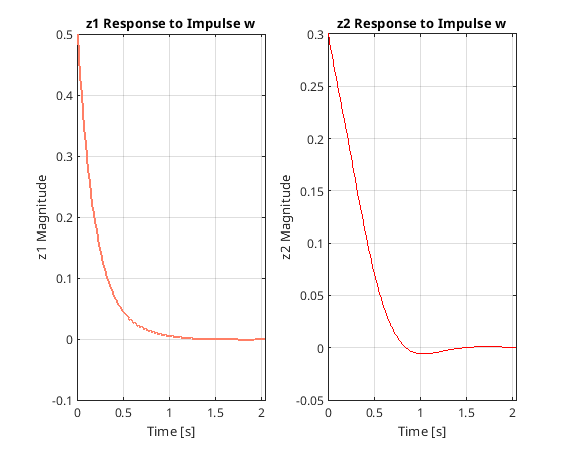
\includegraphics{zResponseHinf.png}
\end{figure}

\subsection{}
\textit{
Generate a max singular value plot of the closed loop system $G_{zw}(s)$ using the command \texttt{sigma}. Does this system amplify (absolute gain $>$ 1) or attenuate (absolute gain $<$ 1) disturbances? Note that the \texttt{sigma} plot generates the gain in dB.
}

Here is my code following the procedure detailed above, I converted from dB to absolute units in the plot function.

\begin{lstlisting}[style=matlabstyle]
[sv,wout] = sigma(hinfSys);

figure;
plot(wout, 10.^(sv/20));
grid on;
title('Max Singular Value at Different Frequencies');
xlabel('Frequency [rad/s]');
ylabel('Absolute Gain [absolute units]');
\end{lstlisting}

These were the results and as you can see the absolute gain is slightly higher than 1 meaning the system amplifies disturbances which does not make a lot of sense to me given the previous results.

\begin{figure}[H]
    \centering
    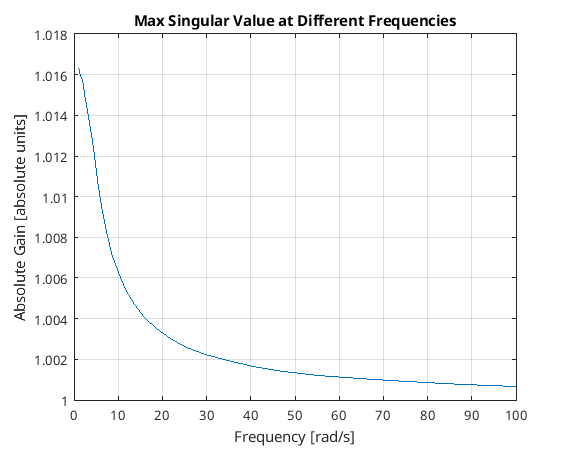
\includegraphics{maxSVhinf.png}
\end{figure}

I wonder if 'sigma' is printing the singular values in decibels because when I use 'hinfnorm' on the system I get 0.1431 and when I plot the singular values without converting I get:

\begin{figure}[H]
    \centering
    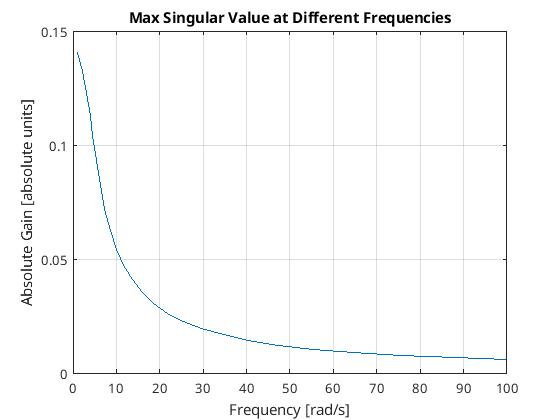
\includegraphics{maxSVhinfDB.png}
\end{figure}


\subsection{}
\textit{
Plot the two control signals $u_1(t)$ and $u_2(t)$ and compute their $L_2$ norms. Which channel requires more input energy?
}

I calculated $u$ using $K$ and the $x$ output from the 'impulse' function:

\begin{lstlisting}[style=matlabstyle]
u = K*x';

figure;
plot(tOut, u(1,:), 'r-', tOut, u(2,:), 'y-');
legend('u1', 'u2');
grid on;
title('Control Signal Response to Impulse Disturbance');
xlabel('Time [s]');
ylabel('Control Signal Magnitude');

disp("u1 L2 Norm: ")
disp(norm(u(1,:),2));

disp("u2 L2 Norm: ")
disp(norm(u(2,:),2));    
\end{lstlisting}

The plot looks like this:

\begin{figure}[H]
    \centering
    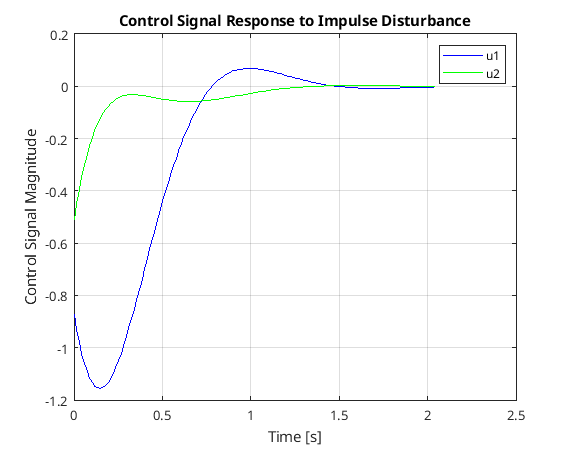
\includegraphics{uResponseHinf.png}
\end{figure}

I computed the $L_2$ norm using Matlab's 'norm' function and got 5.6361 for u1 and 1.0919 for u2 which makes sense looking at the plot there's definitely more area under the curve for u1 and I think this shows that this input channel requires a stronger response to deal with that disturbance.

\section{$H_2$ State Feedback Control}
\textit{
In this problem, you will implement the $H_2$ LMI synthesis approach and design a feedback controller for the DC-8 example that was presented in class the previous week in the $H_\infty$ state feedback example. The MATLAB code to set up the system matrices will be provided.
}

\subsection{}
\textit{
Implement the $H_2$ LMI conditions derived in lecture for the feasibility problem given a prescribed attenuation level $\|G(s)\|_2 < \gamma$ as a function using the LMI Toolbox in MATLAB. Design $\gamma$ for the $H_2$ controller to match the control energy ($L_2$ norm) for an equivalent $H_\infty$ controller with attenuation level $\gamma = 2.5$.
}

\subsection{}
\textit{
Generate the resulting singular value bode plots of the closed loop systems and the responses of the state $x$ due to an impulse in the yaw disturbance $r_g$ for both the $H_2$ and $H_\infty$ controllers and compare both sets of plots.
}

\subsection{}
\textit{
For a white noise yaw disturbance $r_g$ of unit intensity, compute the average power in the states for each of the closed loop systems and compare.
}

\section{$H_\infty$ Observer Design}
\textit{
Consider the standard general LTI system with $D_{11} = D_{12} = 0$,
\[
\dot{x} = Ax + B_2u + B_1w
\]
\[
z = C_1x
\]
\[
y = C_2x + D_{21}w + D_{22}u
\]
with state $x$, measured output $y$, control input $u$, disturbance $w$, and the regulated outputs $z$. For this system, we introduce a full-order state observer in the following form:
\[
\dot{\hat{x}} = A\hat{x} + B_2u + L(C_2\hat{x} + D_{22}u - y)
\]
where $\hat{x}$ is the state observation and $L$ is the observer gain. The estimate of the regulated outputs is given by $\hat{z} = C_1\hat{x}$, which is desired to have as small as possible influence from the disturbance $w$.
}

\subsection{}
\textit{
Show that for $e(t) = x(t) - \hat{x}(t)$ and $\tilde{z}(t) = z(t) - \hat{z}(t)$, the resulting observation error equation is given by
\[
\dot{e} = (A + LC_2)e + (B_1 + LD_{21})w
\]
\[
\tilde{z} = C_1e
\]
and has closed loop transfer function $G_{\tilde{z}w} = C_1[sI - (A + LC_2)]^{-1}(B_1 + LD_{21})$ from $w \rightarrow \tilde{z}$.
}

\subsection{}
\textit{
Consider the following problem: Given the system in (a) and a positive scalar $\gamma$, find a matrix $L$ such that $\|G_{\tilde{z}w}\|_\infty < \gamma$. Prove that this problem has a solution if and only if there exists a matrix $W$ and a positive definite matrix $P > 0$ and the constraint
\[
\begin{pmatrix}
A^TP + PA + C_2^TWC_2 & PB_1 + WD_{21} & C_1^T \\
(PB_1 + WD_{21})^T & -\gamma I & 0 \\
C_1 & 0 & -\gamma I
\end{pmatrix} < 0
\]
holds. When such a pair of matrices $W$ and $P$ are found, the solution to the problem is given as $L = P^{-1}W$.
}

\subsection{}
\textit{
Design an $H_\infty$ observer according to the above approach such that $\|G_{\tilde{z}w}\|_\infty < 0.1$ for the system in Problem 1. Assume that
\[
C_2 = \begin{pmatrix} 1 & 0 & 0 \\ 0 & 0 & 1 \end{pmatrix}, \quad D_{21} = \begin{pmatrix} 0 \\ 1 \end{pmatrix}.
\]
Provide plots of the error states $e_1(t)$, $e_2(t)$, and $e_3(t)$ for 2 seconds for an impulse input in $w$.
}

\end{document}